\documentclass[a4page]{exam}
\usepackage{geometry}
\usepackage[table]{xcolor}
\usepackage{amsmath, amsfonts}
\usepackage{amsmath}
\usepackage{amssymb}
\usepackage{geometry}
\usepackage{tabularx}
\usepackage{hyperref}
\usepackage{tikz}

\usetikzlibrary{shapes,snakes}
\usetikzlibrary{automata,positioning,arrows}

\newcommand{\Str}[1]{\mathtt{#1}}

\title{Homework 2}
\author{CS 212 Nature of Computation\\Habib University\\Fall 2021}
\date{Due: 2359h on Sunday, 24 October}

\begin{document}
\maketitle
\thispagestyle{empty}

\noindent\rule{\textwidth}{1pt}

\begin{questions}
\question[10] Prove that $\{wtw | \hspace{1mm} w,t \in \{0,1\}^+\}$ is not regular.
\\
\\
L= $\{wtw | \hspace{1mm} w,t \in \{0,1\}^+\}$\\
 To prove that L is not a regular language, we will use a proof by contradiction. Assume
that L is a regular language. Then by the Pumping Lemma for Regular Languages,
there exists a pumping length p for L such that for any string $s \in L$  where $|s| \geq p $ ,
$s = xyz$ subject to the following conditions:\\
(a) $|y| > 0$\\
(b) $|xy| \leq p $\\
(c) $\forall i > 0, xy^i z \in L$.\\
Choose s = $0^p110^p1$. Clearly s $\in$ L with $w = 0^p1$ and t = 1, and $|s| \geq p$. By condition
(b), it is obvious that xy is composed only of zeros, and further, by (a) and (b), it
follows that y = 0k
for some k $\geq$ 0. By condition (c), we can take any i and $xy^i$
z will
be in L. Taking i = 2, then $xy^2$
$z \in L$. $xy^2$
z = xyyz = $0^{(p+k)}110^p1.$ There is no way
that this string can be divided into wtw as required to be in L, thus $xy^2 z \notin L$. This is
a contradiction with condition (c) of the pumping lemma. Therefore the assumption
that L is a regular language is incorrect and thus L is not a regular language.

\question Given $L = \{0^i1^j2^k | \hspace{1mm} i,j,k \geq 0 \text{ and } i \neq 1 \text{ or } j = k\}$, show that 
  \begin{parts}
  \part[10] $L$ is not regular.
  \part[10] The pumping lemma for regular languages applies to $L$. That is, show that there is some $p$ such that if $s\in L$ and $|s| > p$, then $s$ can be written as $xyz$ where $|y| > 0, |xy| \le p$, and for each $i \ge 0, xy^iz \in L$.\\ 
    \textit{Note: This shows that the converse of the pumping lemma is false.}
  \end{parts}
a) L is not regular and it cannot be proved using pumping lemma, it can be proved using closure properties.

\question Consider the grammar $G = (V,\Sigma, R, S)$ where $V = \{S,A\}$; $\Sigma = \{\Str{a},\Str{b}\}$; and $R$ contains the following rules:
  \begin{eqnarray*}
    S &\rightarrow& \Str{a}\ A\ \Str{a} \mid \Str{b}\ A\ \Str{b} \mid \epsilon\\
    A &\rightarrow& SS.
  \end{eqnarray*}
  \begin{parts}
  \part[5] Which strings of $L(G)$ can be produced by derivations of four or fewer steps?
  \part[5] Give a derivation of $\Str{baabbb}$ in $G$.
  \part[5] Construct the parse tree of the derivation from the previous part.
  \part[5] Describe $L(G)$ in English?
  \end{parts}

(a)
\\
  $S$ $\rightarrow$  $aAa$ $\rightarrow$ $aSSa$ \\
  $S$ $\rightarrow$  $bAb$ $\rightarrow$ $bSSb$ \\
  S $\rightarrow$ $\in$
 \\
(b)
\\
  S $\rightarrow$ bAb\\
  $\rightarrow$ bSSb\\
  $\rightarrow$ baAab\\
  $\rightarrow$ baSSab\\
  $\rightarrow$ baAabAbb\\
  $\rightarrow$ baSSabSSbb\\
  $\rightarrow$ baabbb\\
(c)
\\

 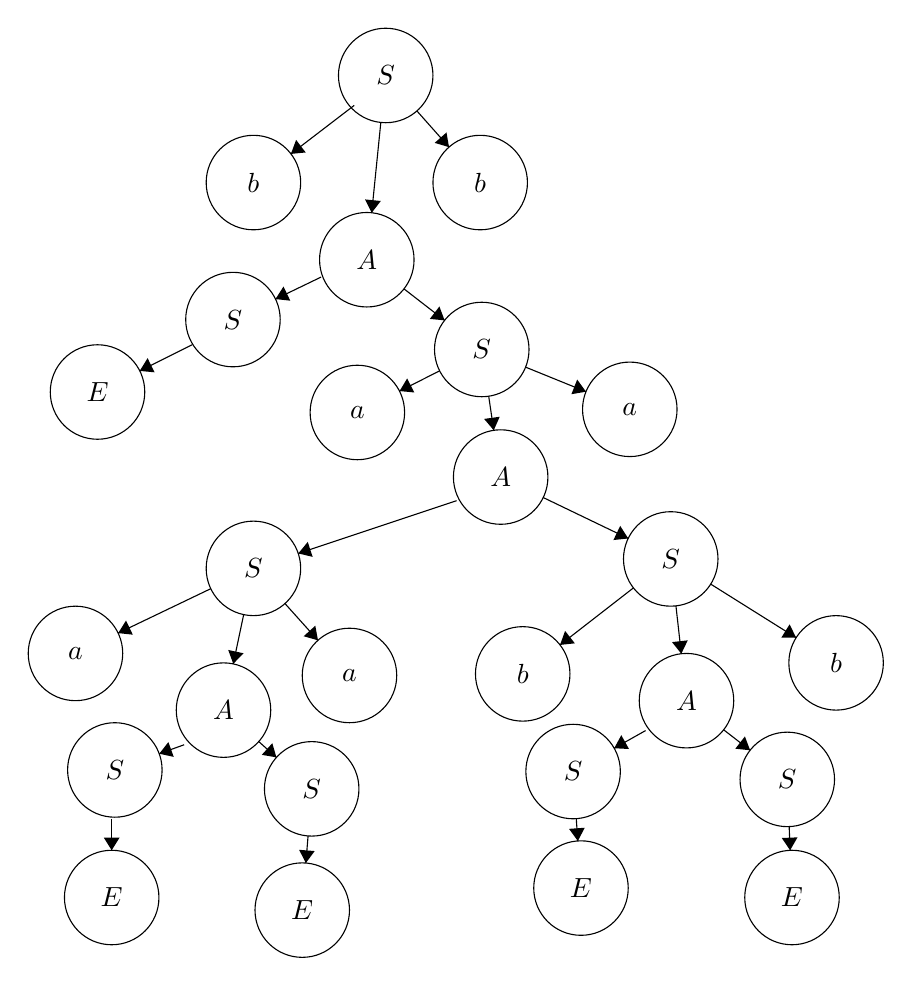
\begin{tikzpicture}[scale=0.2]
\tikzstyle{every node}+=[inner sep=0pt]
\draw [black] (38.7,-4.1) circle (3);
\draw (38.7,-4.1) node {$S$};
\draw [black] (30.3,-10.9) circle (3);
\draw (30.3,-10.9) node {$b$};
\draw [black] (44.7,-10.9) circle (3);
\draw (44.7,-10.9) node {$b$};
\draw [black] (37.5,-15.8) circle (3);
\draw (37.5,-15.8) node {$A$};
\draw [black] (29,-19.6) circle (3);
\draw (29,-19.6) node {$S$};
\draw [black] (20.4,-24.2) circle (3);
\draw (20.4,-24.2) node {$E$};
\draw [black] (44.8,-21.5) circle (3);
\draw (44.8,-21.5) node {$S$};
\draw [black] (36.9,-25.5) circle (3);
\draw (36.9,-25.5) node {$a$};
\draw [black] (46,-29.6) circle (3);
\draw (46,-29.6) node {$A$};
\draw [black] (54.2,-25.3) circle (3);
\draw (54.2,-25.3) node {$a$};
\draw [black] (30.3,-35.4) circle (3);
\draw (30.3,-35.4) node {$S$};
\draw [black] (19,-40.8) circle (3);
\draw (19,-40.8) node {$a$};
\draw [black] (28.4,-44.4) circle (3);
\draw (28.4,-44.4) node {$A$};
\draw [black] (36.4,-42.2) circle (3);
\draw (36.4,-42.2) node {$a$};
\draw [black] (56.8,-34.8) circle (3);
\draw (56.8,-34.8) node {$S$};
\draw [black] (47.4,-42.1) circle (3);
\draw (47.4,-42.1) node {$b$};
\draw [black] (57.8,-43.8) circle (3);
\draw (57.8,-43.8) node {$A$};
\draw [black] (67.3,-41.4) circle (3);
\draw (67.3,-41.4) node {$b$};
\draw [black] (21.5,-48.2) circle (3);
\draw (21.5,-48.2) node {$S$};
\draw [black] (21.3,-56.3) circle (3);
\draw (21.3,-56.3) node {$E$};
\draw [black] (34,-49.4) circle (3);
\draw (34,-49.4) node {$S$};
\draw [black] (33.4,-57.1) circle (3);
\draw (33.4,-57.1) node {$E$};
\draw [black] (50.6,-48.3) circle (3);
\draw (50.6,-48.3) node {$S$};
\draw [black] (51.1,-55.7) circle (3);
\draw (51.1,-55.7) node {$E$};
\draw [black] (64.2,-48.8) circle (3);
\draw (64.2,-48.8) node {$S$};
\draw [black] (64.5,-56.3) circle (3);
\draw (64.5,-56.3) node {$E$};
\draw [black] (36.7,-6) -- (32.68,-9.08);
\fill [black] (32.68,-9.08) -- (33.62,-8.99) -- (33.01,-8.19);
\draw [black] (40.68,-6.35) -- (42.72,-8.65);
\fill [black] (42.72,-8.65) -- (42.56,-7.72) -- (41.81,-8.38);
\draw [black] (38.39,-7.08) -- (37.81,-12.82);
\fill [black] (37.81,-12.82) -- (38.39,-12.07) -- (37.39,-11.97);
\draw [black] (34.6,-16.9) -- (31.7,-18.3);
\fill [black] (31.7,-18.3) -- (32.64,-18.4) -- (32.21,-17.5);
\draw [black] (26.4,-21.2) -- (23.08,-22.86);
\fill [black] (23.08,-22.86) -- (24.02,-22.95) -- (23.58,-22.05);
\draw [black] (39.86,-17.65) -- (42.44,-19.65);
\fill [black] (42.44,-19.65) -- (42.11,-18.77) -- (41.5,-19.56);
\draw [black] (42.12,-22.86) -- (39.58,-24.14);
\fill [black] (39.58,-24.14) -- (40.52,-24.23) -- (40.06,-23.34);
\draw [black] (45.24,-24.47) -- (45.56,-26.63);
\fill [black] (45.56,-26.63) -- (45.94,-25.77) -- (44.95,-25.91);
\draw [black] (47.58,-22.62) -- (51.42,-24.18);
\fill [black] (51.42,-24.18) -- (50.86,-23.41) -- (50.49,-24.34);
\draw [black] (43.2,-31.1) -- (33.15,-34.45);
\fill [black] (33.15,-34.45) -- (34.06,-34.67) -- (33.75,-33.72);
\draw [black] (48.7,-30.9) -- (54.1,-33.5);
\fill [black] (54.1,-33.5) -- (53.59,-32.7) -- (53.16,-33.6);
\draw [black] (29.68,-38.34) -- (29.02,-41.46);
\fill [black] (29.02,-41.46) -- (29.67,-40.79) -- (28.7,-40.58);
\draw [black] (27.59,-36.69) -- (21.71,-39.51);
\fill [black] (21.71,-39.51) -- (22.64,-39.61) -- (22.21,-38.71);
\draw [black] (32.3,-37.63) -- (34.4,-39.97);
\fill [black] (34.4,-39.97) -- (34.23,-39.04) -- (33.49,-39.71);
\draw [black] (54.43,-36.64) -- (49.77,-40.26);
\fill [black] (49.77,-40.26) -- (50.71,-40.16) -- (50.09,-39.37);
\draw [black] (57.13,-37.78) -- (57.47,-40.82);
\fill [black] (57.47,-40.82) -- (57.88,-39.97) -- (56.88,-40.08);
\draw [black] (59.34,-36.4) -- (64.76,-39.8);
\fill [black] (64.76,-39.8) -- (64.35,-38.95) -- (63.82,-39.8);
\draw [black] (30.64,-46.4) -- (31.76,-47.4);
\fill [black] (31.76,-47.4) -- (31.5,-46.5) -- (30.83,-47.24);
\draw [black] (33.77,-52.39) -- (33.63,-54.11);
\fill [black] (33.63,-54.11) -- (34.19,-53.35) -- (33.2,-53.27);
\draw [black] (25.9,-46.6) -- (24.32,-47.17);
\fill [black] (24.32,-47.17) -- (25.24,-47.37) -- (24.9,-46.43);
\draw [black] (21.3,-51.3) -- (21.3,-53.3);
\fill [black] (21.3,-53.3) -- (21.8,-52.5) -- (20.8,-52.5);
\draw [black] (55.2,-45.7) -- (53.21,-46.82);
\fill [black] (53.21,-46.82) -- (54.15,-46.87) -- (53.66,-45.99);
\draw [black] (60.16,-45.65) -- (61.84,-46.95);
\fill [black] (61.84,-46.95) -- (61.51,-46.07) -- (60.9,-46.85);
\draw [black] (64.32,-51.8) -- (64.38,-53.3);
\fill [black] (64.38,-53.3) -- (64.85,-52.48) -- (63.85,-52.52);
\draw [black] (50.8,-51.29) -- (50.9,-52.71);
\fill [black] (50.9,-52.71) -- (51.34,-51.87) -- (50.34,-51.94);
\end{tikzpicture}
\\(d) We can say that this language pumps from top to middle and each terminal occur in pairs always as we looking at the pattern of strings produced.


\question[10] Convert the following context-free grammar to Chomsky Normal Form:
  \begin{eqnarray*}
    S &\rightarrow& A\ S\ B\\
    A &\rightarrow& \Str{a}\ A\ S\ \mid\  \Str{a}\ \mid\ \epsilon \\
    B &\rightarrow& S\ \Str{b}\ S\ \mid\ A\ \mid\ \Str{b}\ \Str{b}.
  \end{eqnarray*}

As we can see the start symbol S is on the right hand side therefore, we will introduce a new start symbol $S_{0}$ $\rightarrow$ S\\
A produces a null element therefore, in order to remove it, the new yield will be\\
$S_{0}$ $\rightarrow S$\\
S $\rightarrow A\ S\ B $\\
    A $\rightarrow \Str{a}\ A\ S\ \mid\  \Str{a}\ S \ \mid\ str{a}$ \\
    B $\rightarrow S\ \Str{b}\ S\ \mid\ A\ \mid\ \epsilon \ \mid \Str{b} \ \Str{b}$.\\
\\
B produces a null element therefore, in order to remove it, the new yield will be\\
$S_{0}$ $\rightarrow S$\\
S $\rightarrow A\ S\ \mid \ A \ S \ B \mid \ S \ B \ \mid \ S  $\\
    A $\rightarrow \Str{a}\ A\ S\ \mid\  \Str{a}\ S \ \mid\ a$ \\
    B $\rightarrow S\ \Str{b}\ S\ \mid\ A\ \mid \Str{b} \ \Str{b}$.\\
\\
B produces A therefore, in order to remove it, the new yield will be\\
$S_{0}$ $\rightarrow S$\\
S $\rightarrow A\ S\ \mid \ A \ S \ B \mid \ S \ B \ \mid \ S  $\\
    A $\rightarrow \Str{a}\ A\ S\ \mid\  \Str{a}\ S \ \mid\ a$ \\
    B $\rightarrow S\ \Str{b}\ S\ \mid\ \Str{b} \ \Str{b}\ \mid \Str{a} \ A \ S \mid \ \Str{a} \ S \ \mid \ \Str{a}$.\\
\\
Now we will remove $S_{0}$ $\rightarrow S$ and it will yield\\
$S_{0}$ $\rightarrow A \ S \ \mid \ A \ S \ B \ \mid S \ B \ \mid \ S$\\
S $\rightarrow A\ S\ \mid \ A \ S \ B \mid \ S \ B \ \mid \ S  $\\
    A $\rightarrow \Str{a}\ A\ S\ \mid\  \Str{a}\ S \ \mid\ a$ \\
    B $\rightarrow S\ \Str{b}\ S\ \mid\ \Str{b} \ \Str{b}\ \mid \Str{a} \ A \ S \mid \ \Str{a} \ S \ \mid \ \Str{a}$.\\
\\
Now we will remove$S \rightarrow S$ and $S_{0}$ $\rightarrow S$ and it will yield\\
$S_{0}$ $\rightarrow A \ S \ \mid \ A \ S \ B \ \mid S \ B $\\
S $\rightarrow A\ S\ \mid \ A \ S \ B \mid \ S \ B   $\\
    A $\rightarrow \Str{a}\ A\ S\ \mid\  \Str{a}\ S \ \mid\ \Str{a}$ \\
    B $\rightarrow S\ \Str{b}\ S\ \mid\ \Str{b} \ \Str{b}\ \mid \Str{a} \ A \ S \mid \ \Str{a} \ S \ \mid \ \Str{a}$.\\
\\
Now we will remove $\Str{a}$, $\Str{b}$ and $B \rightarrow bb$ from A and B as they appear on right side\\
$S_{0}$ $\rightarrow A \ S \ \mid \ A \ S \ B \ \mid S \ B $\\
S $\rightarrow A\ S\ \mid \ A \ S \ B \mid \ S \ B   $\\
    A $\rightarrow \ X\ A\ S\ \mid\  X \ S \ \mid\ \Str{a}$ \\
    B $\rightarrow S\ Y \ S\ \mid\ V\ V\ \mid X \ A \ S \mid \ X \ S \ \mid \ \Str{a}$.\\
X $\rightarrow$ a\\
Y $\rightarrow$ b\\
Z $\rightarrow$ b\\
\\
$S_{0}$ $\rightarrow \ A \ S \ B $ has more than two symbols, inorder to correct its yield, it will be\\
$S_{0}$ $\rightarrow A \ S \ \mid \ P \ B \ \mid S \ B $\\
S $\rightarrow A\ S\ \mid \ A \ S \ B \mid \ S \ B   $\\
    A $\rightarrow \ X\ A\ S\ \mid\  X \ S \ \mid\ \Str{a}$ \\
    B $\rightarrow S\ Y \ S\ \mid\ V\ V\ \mid X \ A \ S \mid \ X \ S \ \mid \ \Str{a}$.\\
X $\rightarrow$ a\\
Y $\rightarrow$ b\\
Z $\rightarrow$ b\\
P $\rightarrow$ AS\\
\\
$S \rightarrow \ A \ S \ B $ has more than two symbols, inorder to correct its yield, it will be\\
$S_{0}$ $\rightarrow A \ S \ \mid \ P \ B \ \mid S \ B $\\
S $\rightarrow A\ S\ \mid \ Q \ B \mid \ S \ B   $\\
    A $\rightarrow \ X\ A\ S\ \mid\  X \ S \ \mid\ \Str{a}$ \\
    B $\rightarrow S\ Y \ S\ \mid\ V\ V\ \mid X \ A \ S \mid \ X \ S \ \mid \ \Str{a}$.\\
X $\rightarrow$ a\\
Y $\rightarrow$ b\\
Z $\rightarrow$ b\\
P $\rightarrow$ AS\\
Q $\rightarrow$ AS\\
\\
$A \rightarrow \ X \ A \ S $ has more than two symbols, inorder to correct its yield, it will be\\
$S_{0}$ $\rightarrow A \ S \ \mid \ P \ B \ \mid S \ B $\\
S $\rightarrow A\ S\ \mid \ Q \ B \mid \ S \ B   $\\
    A $\rightarrow \ R\ S\ \mid\  X \ S \ \mid\ \Str{a}$ \\
    B $\rightarrow S\ Y \ S\ \mid\ V\ V\ \mid X \ A \ S \mid \ X \ S \ \mid \ \Str{a}$.\\
X $\rightarrow$ a\\
Y $\rightarrow$ b\\
Z $\rightarrow$ b\\
P $\rightarrow$ AS\\
Q $\rightarrow$ AS\\
R $\rightarrow$ XA\\
\\
$B \rightarrow \ S \ Y \ S $  and $B \rightarrow \ S \ Y \ S $ has more than two symbols, inorder to correct its yield, it will be\\
$S_{0}$ $\rightarrow A \ S \ \mid \ P \ B \ \mid S \ B $\\
S $\rightarrow A\ S\ \mid \ Q \ B \mid \ S \ B   $\\
    A $\rightarrow \ R\ S\ \mid\  X \ S \ \mid\ \Str{a}$ \\
    B $\rightarrow T \ S\ \mid\ V\ V\ \mid X \ A \ S \mid \ X \ S \ \mid \ \Str{a}$.\\
X $\rightarrow$ a\\
Y $\rightarrow$ b\\
Z $\rightarrow$ b\\
P $\rightarrow$ AS\\
Q $\rightarrow$ AS\\
R $\rightarrow$ XA\\
T $\rightarrow$ SY\\
\\
$B \rightarrow \ X \ A \ S $ has more than two symbols, inorder to correct its yield, it will be\\
$S_{0}$ $\rightarrow A \ S \ \mid \ P \ B \ \mid S \ B $\\
S $\rightarrow A\ S\ \mid \ Q \ B \mid \ S \ B   $\\
    A $\rightarrow \ R\ S\ \mid\  X \ S \ \mid\ \Str{a}$ \\
    B $\rightarrow T \ S\ \mid\ V\ V\ \mid \ U \ S \mid \ X \ S \ \mid \ \Str{a}$.\\
X $\rightarrow$ a\\
Y $\rightarrow$ b\\
Z $\rightarrow$ b\\
P $\rightarrow$ AS\\
Q $\rightarrow$ AS\\
R $\rightarrow$ XA\\
T $\rightarrow$ SY\\


Reference: https://www.geeksforgeeks.org/converting-context-free-grammar-chomsky-normal-form/

\question Give an unambiguous context-free grammar and then construct a pushdown automaton for each of the following languages.
  \begin{parts}
  \part[20] $L = \{a^n b^m c^k \mid n, m, k > 0, k = n + m \}$ over $\Sigma = \{a, b, c\}$.
  \part[20] $A = \{w \mid \text{the number of $a$'s is at least the number of $b$'s in $w$} \}$ over $\Sigma = \{a, b\}$.
  \end{parts}
part a 
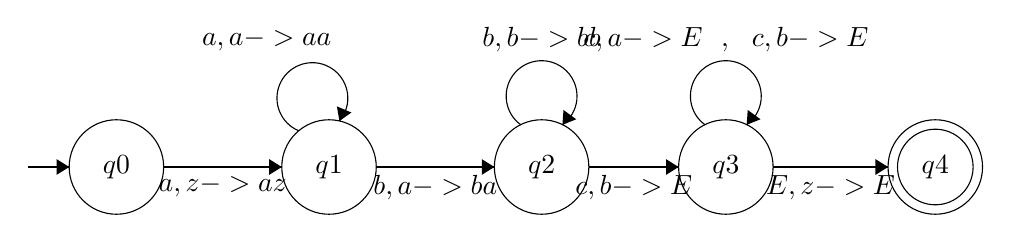
\begin{tikzpicture}[scale=0.2]
\tikzstyle{every node}+=[inner sep=0pt]
\draw [black] (9.2,-17.3) circle (3);
\draw (9.2,-17.3) node {$q0$};
\draw [black] (22.7,-17.3) circle (3);
\draw (22.7,-17.3) node {$q1$};
\draw [black] (36.2,-17.3) circle (3);
\draw (36.2,-17.3) node {$q2$};
\draw [black] (47.9,-17.3) circle (3);
\draw (47.9,-17.3) node {$q3$};
\draw [black] (61.2,-17.3) circle (3);
\draw (61.2,-17.3) node {$q4$};
\draw [black] (61.2,-17.3) circle (2.4);
\draw [black] (3.6,-17.3) -- (6.2,-17.3);
\fill [black] (6.2,-17.3) -- (5.4,-16.8) -- (5.4,-17.8);
\draw [black] (12.2,-17.3) -- (19.7,-17.3);
\fill [black] (19.7,-17.3) -- (18.9,-16.8) -- (18.9,-17.8);
\draw (15.95,-17.8) node [below] {$a,z->az$};
\draw [black] (20.786,-15.005) arc (247.57043:-40.42957:2.25);
\draw (18.74,-9.99) node [above] {$a,a->aa$};
\fill [black] (23.36,-14.38) -- (24.12,-13.84) -- (23.2,-13.45);
\draw [black] (25.7,-17.3) -- (33.2,-17.3);
\fill [black] (33.2,-17.3) -- (32.4,-16.8) -- (32.4,-17.8);
\draw (29.45,-17.8) node [below] {$b,a->ba$};
\draw [black] (34.877,-14.62) arc (234:-54:2.25);
\draw (36.2,-10.05) node [above] {$b,b->bb$};
\fill [black] (37.52,-14.62) -- (38.4,-14.27) -- (37.59,-13.68);
\draw [black] (39.2,-17.3) -- (44.9,-17.3);
\fill [black] (44.9,-17.3) -- (44.1,-16.8) -- (44.1,-17.8);
\draw (42.05,-17.8) node [below] {$c,b->E$};
\draw [black] (46.577,-14.62) arc (234:-54:2.25);
\draw (47.9,-10.05) node [above] {$c,a->E\mbox{ }\mbox{ },\mbox{ }\mbox{ }c,b->E$};
\fill [black] (49.22,-14.62) -- (50.1,-14.27) -- (49.29,-13.68);
\draw [black] (50.9,-17.3) -- (58.2,-17.3);
\fill [black] (58.2,-17.3) -- (57.4,-16.8) -- (57.4,-17.8);
\draw (54.55,-17.8) node [below] {$E,z->E$};
\end{tikzpicture}\\
\\
Consider l=1 m=3 $\implies$ n=4\\
s(q0, abbbcccc, z)= s(q1, bbbcccc, az)\\
s(q0, abbbcccc, z)   = s(q2, bbcccc, baz)\\
s(q0, abbbcccc, z)   = s(q2, bcccc, bbaz)\\
s(q0, abbbcccc, z)   = s(q2, cccc, bbbaz)\\
s(q0, abbbcccc, z)   = s(q3, ccc, bbaz)\\
s(q0, abbbcccc, z)   = s(q2, cc, bbaz)\\
s(q0, abbbcccc, z)   = s(q2, c, baz)\\
s(q0, abbbcccc, z)   = s(q2, E, z)\\ and so on.\\
\\
 Part b


  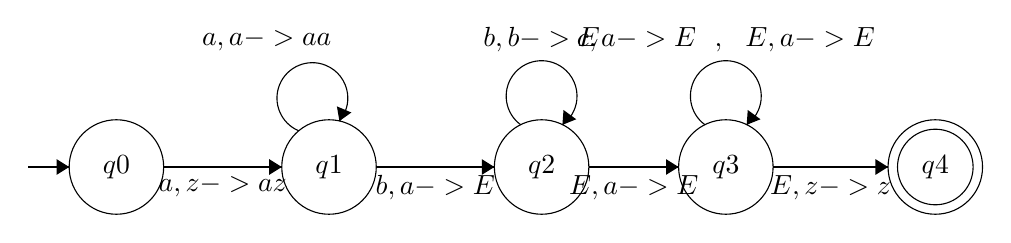
\begin{tikzpicture}[scale=0.2]
\tikzstyle{every node}+=[inner sep=0pt]
\draw [black] (9.2,-17.3) circle (3);
\draw (9.2,-17.3) node {$q0$};
\draw [black] (22.7,-17.3) circle (3);
\draw (22.7,-17.3) node {$q1$};
\draw [black] (36.2,-17.3) circle (3);
\draw (36.2,-17.3) node {$q2$};
\draw [black] (47.9,-17.3) circle (3);
\draw (47.9,-17.3) node {$q3$};
\draw [black] (61.2,-17.3) circle (3);
\draw (61.2,-17.3) node {$q4$};
\draw [black] (61.2,-17.3) circle (2.4);
\draw [black] (3.6,-17.3) -- (6.2,-17.3);
\fill [black] (6.2,-17.3) -- (5.4,-16.8) -- (5.4,-17.8);
\draw [black] (12.2,-17.3) -- (19.7,-17.3);
\fill [black] (19.7,-17.3) -- (18.9,-16.8) -- (18.9,-17.8);
\draw (15.95,-17.8) node [below] {$a,z->az$};
\draw [black] (20.786,-15.005) arc (247.57043:-40.42957:2.25);
\draw (18.74,-9.99) node [above] {$a,a->aa$};
\fill [black] (23.36,-14.38) -- (24.12,-13.84) -- (23.2,-13.45);
\draw [black] (25.7,-17.3) -- (33.2,-17.3);
\fill [black] (33.2,-17.3) -- (32.4,-16.8) -- (32.4,-17.8);
\draw (29.45,-17.8) node [below] {$b,a->E$};
\draw [black] (34.877,-14.62) arc (234:-54:2.25);
\draw (36.2,-10.05) node [above] {$b,b->E$};
\fill [black] (37.52,-14.62) -- (38.4,-14.27) -- (37.59,-13.68);
\draw [black] (39.2,-17.3) -- (44.9,-17.3);
\fill [black] (44.9,-17.3) -- (44.1,-16.8) -- (44.1,-17.8);
\draw (42.05,-17.8) node [below] {$E,a->E$};
\draw [black] (46.577,-14.62) arc (234:-54:2.25);
\draw (47.9,-10.05) node [above] {$c,a->E\mbox{ }\mbox{ },\mbox{ }\mbox{ }E,a->E$};
\fill [black] (49.22,-14.62) -- (50.1,-14.27) -- (49.29,-13.68);
\draw [black] (50.9,-17.3) -- (58.2,-17.3);
\fill [black] (58.2,-17.3) -- (57.4,-16.8) -- (57.4,-17.8);
\draw (54.55,-17.8) node [below] {$E,z->z$};
\end{tikzpicture}
  
\end{questions}

\noindent\rule{\textwidth}{1pt}\\\vspace{1pt}
\end{document}

%%% Local Variables:
%%% mode: latex
%%% TeX-master: t
%%% End:
